\section{飞机增稳控制}
\subsection{飞行品质评估}
将飞机线化小扰动方程纵横分离,得到状态矩阵
$$
A_{\text{lon}}=
\begin{pmatrix}
-0.01538&0.0439&-7.8391&-9.8025\\
-0.04381&0.1204&203.051&-0.3784\\
0.0012&-0.0022&-0.4031&0\\
0&0&1&0
\end{pmatrix}
,
B_{\text{lon}}=
\begin{pmatrix}
2.0701&9.5705\\
-88.0560&0\\
-20.5780&-0.1436\\
0&0
\end{pmatrix}
$$
$$
A_{\text{lat}}=
\begin{pmatrix}
-0.4563&7.8391&-203.0510&9.8025&0\\
-0.1379&-2.9973&2.1335&0&0\\
0.0863&0.0125&-0.7356&0&0\\
0&1&0.0386&0&0\\
0&0&1.0007&0&0
\end{pmatrix}
,
B_{\text{lat}}=
\begin{pmatrix}
12.2129&14.4466\\
-84.7711&15.1058\\
-3.2553&-6.8365\\
0&0\\
0&0
\end{pmatrix}
$$
\subsubsection{纵向飞行品质}
计算纵向状态矩阵$A_{\text{lon}}$的特征值:
$$
\begin{aligned}
\lambda_{1,2}&=-0.1946\pm 0.6453\mi\\
\lambda_{3,4}&=-0.0086\pm 0.0414\mi
\end{aligned}
$$
计算得到纵向模态特性
$$
\omega_{sp}=0.6740\ \ ,\ \ \zeta_{sp}=0.2887
$$
$$
\omega_{p}=0.0423\ \ ,\ \ \zeta_{p}=0.2036
$$
计算单位迎角过载
$$
\mmm=-\mmc_{\text{lon}}\mma_{\text{lon}}^{-1}\mmb_{\text{lon}}+\mmd_{\text{lon}}
$$
$$
\frac{\diff n}{\diff\alpha}=\frac{m_{11}}{m_{21}}=28.92
$$
与GJB-185-1986标准进行对比,如下表所示;
\begin{table}[!h]
\centering
\caption{纵向飞行品质参数对比}
\begin{tabular}{@{}cccc@{}}
\toprule
模态&参数 & 计算值 & 一级飞行品质标准 \\ \midrule
\multirow{2}{*}{短周期}&$\frac{\omega_{sp}^2}{\diff n/\diff \alpha}$ & 0.0157 & $0.085\sim3.6$ \\
&$\zeta_{sp}$ & 0.2887 & $0.3\sim2.0$ \\ \midrule
长周期&$\zeta_p$ & 0.0423 & $>0.04$ \\ \bottomrule
\end{tabular}
\end{table}

\subsubsection{横航向飞行品质}
计算横航向矩阵$A_{\text{lat}}$特征值:
$$
\begin{aligned}
\lambda_0&=0\\
\lambda_{1}&=-2.8908\\
\lambda_{2,3}&=-0.6576\pm 4.2816\mi\\
\lambda_{4}&=0.0168
\end{aligned}
$$
计算得到纵向模态特性,与标准进行对比,如下表所示:
\begin{table}[!h]
\centering
\caption{横航向飞行品质参数对比}
\begin{tabular}{@{}cccc@{}}
\toprule
模态&参数 & 计算值 & 一级飞行品质标准 \\ \midrule
滚转收敛&$\tau$&0.2398&$<1.0$\\ \midrule
\multirow{2}{*}{荷兰滚}&$\omega_{dr}$ & 4.3318 & $>1.0$ \\
&$\zeta_{dr}$ & 0.1518 & $>0.08$ \\ \midrule
螺旋&$T_2$ &41.3753 & $>20$ \\ \bottomrule
\end{tabular}
\end{table}
\clearpage
\subsection{增稳系统设计}
对比飞行品质可以看出,飞机横航向符合一级飞行品质,无需增稳。
纵向长周期符合飞行品质要求,短周期角频率和阻尼比不足,需要增加短周期角频率。

绘制$\de-\theta$的根轨迹,如下图所示。
\begin{figure}[!h]
\centering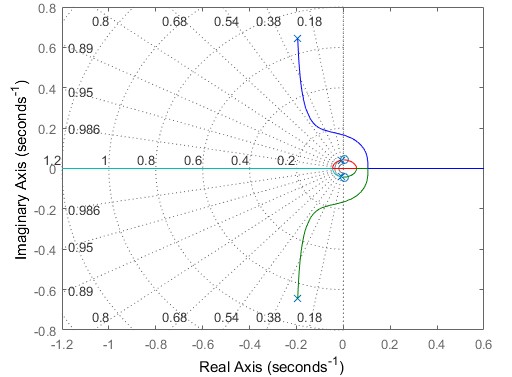
\includegraphics[width=0.8\textwidth]{rl.png}
\caption{$\de-\theta$的根轨迹}
\label{rl}
\end{figure}

若要使短周符合一级飞行品质标准,短周期频率至少为$\sqrt{0.085\d n/\d\alpha}=1.57$。
从根轨迹图中可以看出,代表短周期的一支根轨迹完全处于范围之外,因此无法使用单一变量反馈来实现增稳。
因此采用全状态反馈的方法进行增稳。

设定纵向短周期角频率和阻尼比分别为
$$\omega_{sp}'=6\ \ ,\ \ \zeta_{sp}'=0.707$$
计算得到对应的特征根
$$R'=-4.2420\pm4.2433i$$
将纵向状态$[\Delta U,\Delta W,q,\Delta\theta]^T$反馈到升降舵$\de$,使用place函数进行极点配置,
短周期极点为$R'$,长周期极点不变,得到反馈增益
$$\mvK=[0.0045,-0.0085,-0.3567,0.0328]^T$$
控制结构如下图所示。

【图】

控制增稳后的根轨迹如下图所示

\clearpage
\section{自动飞行仿真}
\subsection{自动导航控制系统}
\clearpage
\subsection{自动飞行仿真}
仿真使用的Simulink模型如下图所示。图中plane model模块为飞机的状态空间模型,Autopilot模块使用状态机,根据飞机的速度,高度和航向确定当前飞行阶段的期望值。
仿真结果如图所示。飞机的迎角,侧滑角和三轴过载通过飞机的体轴系速度及姿态角算出。

\begin{figure}[!h]
\centering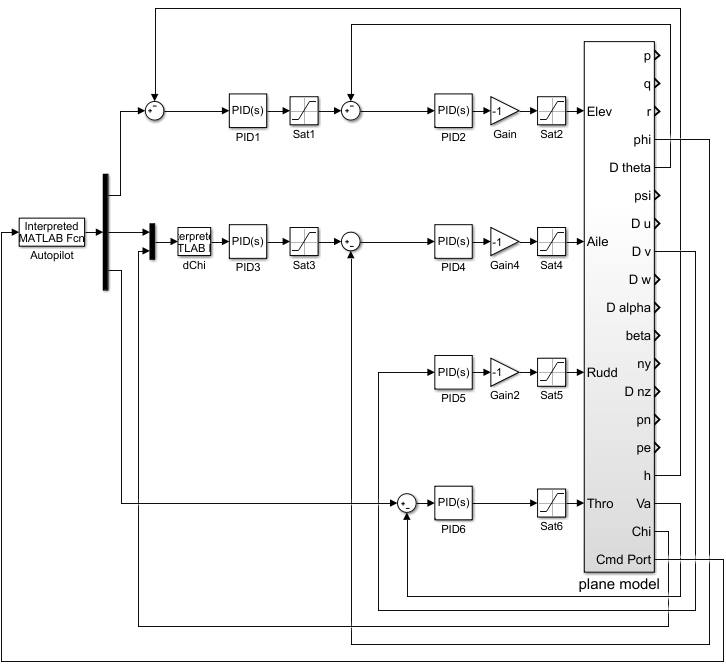
\includegraphics[width=1.1\textwidth]{sim.png}
\caption{仿真系统模型}
\label{sim}
\end{figure}

\begin{figure}[!h]
\centering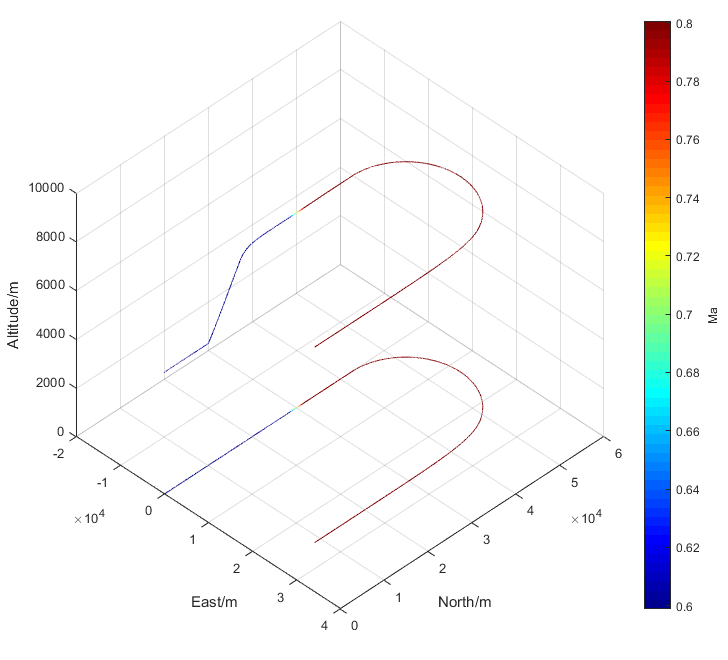
\includegraphics[width=1.1\textwidth]{course.png}
\caption{飞机飞行航迹及其在水平面的投影}
\label{course}
\end{figure}

\begin{figure}[!h]
\centering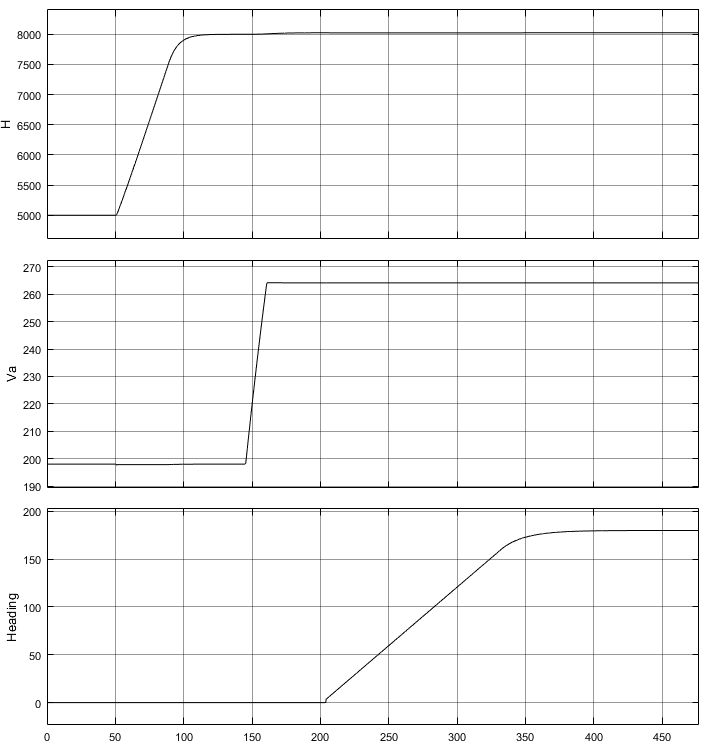
\includegraphics[width=1.1\textwidth]{reshvh.png}
\caption{高度,速度,航向曲线}
\label{course}
\end{figure}

\begin{figure}[!h]
\centering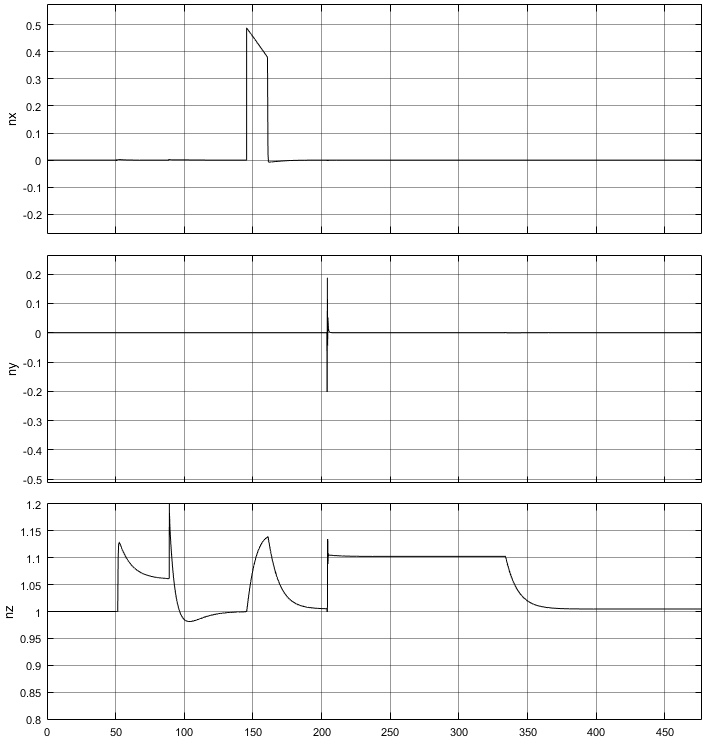
\includegraphics[width=1.1\textwidth]{resn.png}
\caption{三轴过载曲线}
\label{course}
\end{figure}

\begin{figure}[!h]
\centering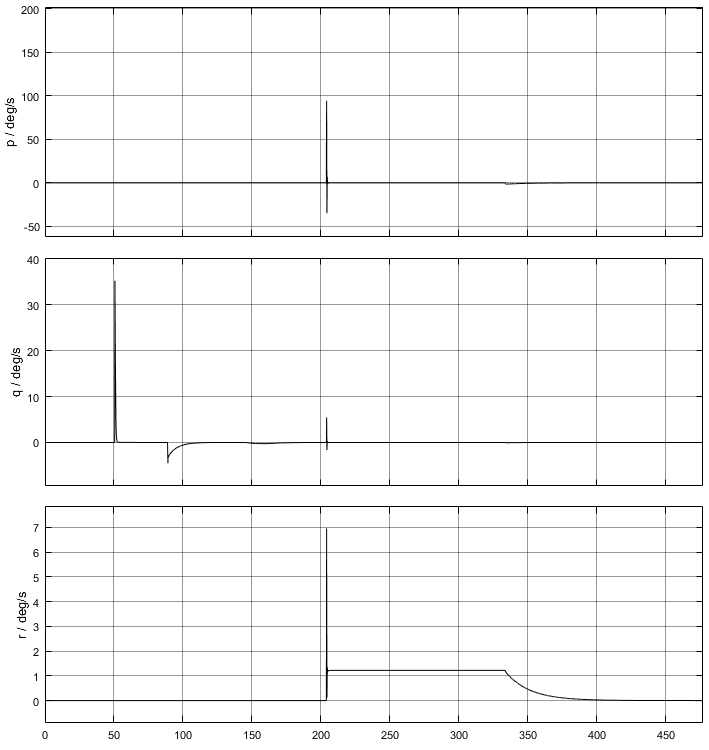
\includegraphics[width=1.1\textwidth]{respqr.png}
\caption{体轴系角速率曲线}
\label{course}
\end{figure}

\begin{figure}[!h]
\centering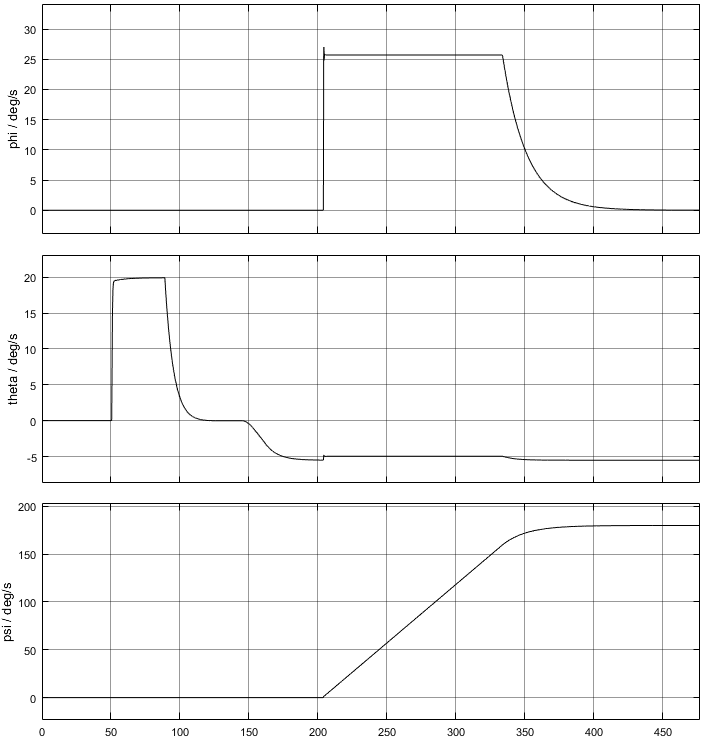
\includegraphics[width=1.1\textwidth]{resptp.png}
\caption{姿态角曲线}
\label{course}
\end{figure}

\begin{figure}[!h]
\centering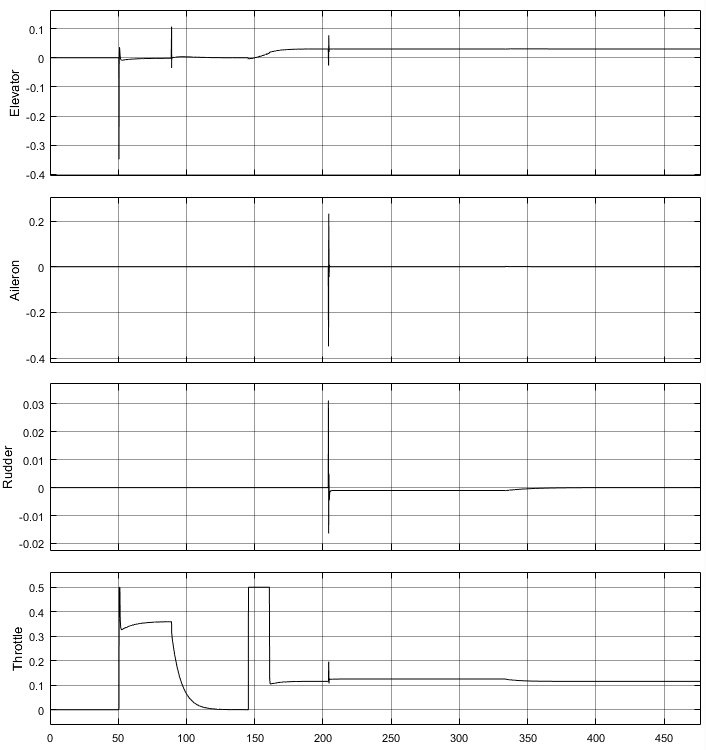
\includegraphics[width=1.1\textwidth]{resctrl.png}
\caption{操纵量输出曲线}
\label{course}
\end{figure}

\endinput
